\documentclass[12pt,notitlepage]{article}
%\usepackage[margin=1in]{geometry}
%	\geometry{
%	top=20mm,
%	bottom=20mm,
%	}
\usepackage[margin=1in]{geometry}              
\usepackage{placeins}
\usepackage{graphicx}
\usepackage{epstopdf}
\usepackage{mathtools}
\usepackage{mathrsfs}
\usepackage{amsmath, amsthm, amssymb, centernot}
\usepackage{subcaption}
\usepackage{booktabs}
\usepackage{multirow}
\usepackage{comment}
\newcommand{\sym}[1] {\ifmmode^{#1} \else\(^{#1}\) \fi}

\DeclareMathOperator{\plim}{plim}

\usepackage{hyperref}
\hypersetup{
    colorlinks,
    citecolor=black,
    filecolor=black,
    linkcolor=blue,
    urlcolor=blue
}
\setlength\parindent{0pt}

\DeclareGraphicsRule{.tif}{png}{.png}{`convert #1 `dirname #1`/`basename #1 .tif`.png}
\pagestyle{plain}
\title{Orbis Data for 4 Countries}
\author{}
\date{}


\begin{document}
\maketitle

\subsection*{Enterprise Survey (India): Standard effects of collateral constraint}


%\begin{figure}[!htpb]
%\centering
%\caption{First stage effect of Court history on collateral requirement of loans}
%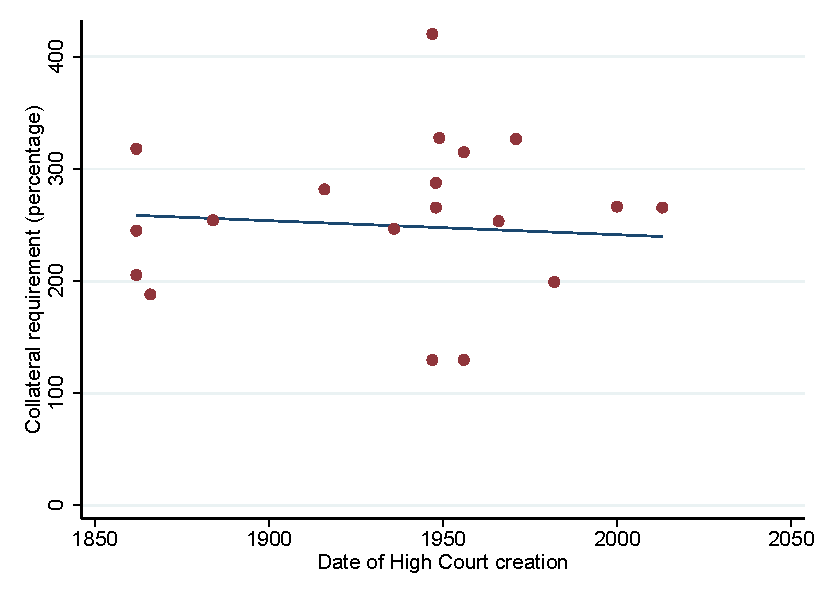
\includegraphics{../Output/Graphs/CourtHist_Colreq.pdf}
%\end{figure}


\begin{table}[htbp]\centering
\def\sym#1{\ifmmode^{#1}\else\(^{#1}\)\fi}
\caption{Collateral constraint and labor share}
\begin{tabular}{l*{2}{c}}
\toprule
                    &\multicolumn{1}{c}{Unconstrained}&\multicolumn{1}{c}{constrained}\\
                    &        mean&        mean\\
\midrule
labor\_share         &      .17071&    .1971271\\
\midrule
Observations        &        2753&         671\\
\bottomrule
\end{tabular}
\end{table}

\pagebreak

\subsection*{Enterprise Survey (India): Non-standard effects of collateral constraint}

\begin{table}[htbp]\centering
\def\sym#1{\ifmmode^{#1}\else\(^{#1}\)\fi}
\caption{Collateral constraint and education of workers}
\begin{tabular}{l*{2}{c}}
\toprule
                    &\multicolumn{1}{c}{Unconstrained}&\multicolumn{1}{c}{constrained}\\
                    &        mean&        mean\\
\midrule
Average years of education&    9.545587&     9.09687\\
\midrule
Observations        &        2753&         671\\
\bottomrule
\end{tabular}
\end{table}

\begin{table}[htbp]\centering
\def\sym#1{\ifmmode^{#1}\else\(^{#1}\)\fi}
\caption{Collateral constraint and training}
\begin{tabular}{l*{2}{c}}
\toprule
                    &\multicolumn{1}{c}{Unconstrained}&\multicolumn{1}{c}{constrained}\\
                    &        mean&        mean\\
\midrule
Firm has formal training program&    1.543046&    1.524112\\
\midrule
Observations        &        3624&         788\\
\bottomrule
\end{tabular}
\end{table}

\begin{table}[htbp]\centering
\def\sym#1{\ifmmode^{#1}\else\(^{#1}\)\fi}
\caption{Collateral constraint and proportion of training towards skilled labor}
\begin{tabular}{l*{2}{c}}
\toprule
                    &\multicolumn{1}{c}{Unconstrained}&\multicolumn{1}{c}{constrained}\\
                    &        mean&        mean\\
\midrule
proportion of formal training towards skilled labor&    .5309755&    .5095277\\
\midrule
Observations        &         832&         192\\
\bottomrule
\end{tabular}
\end{table}


\pagebreak

%\begin{table}[htbp]\centering
\def\sym#1{\ifmmode^{#1}\else\(^{#1}\)\fi}
\caption{First stage of Court History on collateral requirement}
\begin{tabular}{l*{1}{c}}
\toprule
                    &\multicolumn{1}{c}{First Stage}\\
\midrule
Year of high court creation&      -0.125\sym{***}\\
                    &    (-72.19)         \\
\addlinespace
Constant            &       491.0\sym{***}\\
                    &    (151.06)         \\
\midrule
Observations        &      816249         \\
\bottomrule
\multicolumn{2}{l}{\footnotesize \textit{t} statistics in parentheses}\\
\multicolumn{2}{l}{\footnotesize \sym{*} \(p<0.05\), \sym{**} \(p<0.01\), \sym{***} \(p<0.001\)}\\
\end{tabular}
\end{table}

%\begin{table}[htbp]\centering
\def\sym#1{\ifmmode^{#1}\else\(^{#1}\)\fi}
\caption{Effect of collateral requirement on productivity of labor}
\begin{tabular}{l*{2}{c}}
\toprule
                    &\multicolumn{1}{c}{OLS}&\multicolumn{1}{c}{IV}\\
\midrule
Collateral requirement&       587.5         &    -15322.3         \\
                    &      (1.45)         &     (-0.16)         \\
\midrule
Observations        &      511579         &      501664         \\
\bottomrule
\multicolumn{3}{l}{\footnotesize \textit{t} statistics in parentheses}\\
\multicolumn{3}{l}{\footnotesize \sym{+} \(p<0.10\), \sym{*} \(p<0.05\), \sym{**} \(p<0.01\), \sym{***} \(p<0.001\)}\\
\end{tabular}
\end{table}

%\begin{table}[htbp]\centering
\def\sym#1{\ifmmode^{#1}\else\(^{#1}\)\fi}
\caption{Effect of collateral requirement on labor share}
\begin{tabular}{l*{2}{c}}
\toprule
                    &\multicolumn{1}{c}{OLS}&\multicolumn{1}{c}{IV}\\
\midrule
Collateral requirement&     24126.5\sym{***}&   1420318.0\sym{***}\\
                    &      (5.55)         &     (16.83)         \\
\midrule
Observations        &      667933         &      655810         \\
\bottomrule
\multicolumn{3}{l}{\footnotesize \textit{t} statistics in parentheses}\\
\multicolumn{3}{l}{\footnotesize \sym{+} \(p<0.10\), \sym{*} \(p<0.05\), \sym{**} \(p<0.01\), \sym{***} \(p<0.001\)}\\
\end{tabular}
\end{table}

%\begin{table}[htbp]\centering
\def\sym#1{\ifmmode^{#1}\else\(^{#1}\)\fi}
\caption{Effect of collateral requirement on wages}
\begin{tabular}{l*{2}{c}}
\toprule
                    &\multicolumn{1}{c}{OLS}&\multicolumn{1}{c}{IV}\\
\midrule
Collateral requirement&       108.8\sym{***}&      2866.7\sym{***}\\
                    &     (44.59)         &     (30.03)         \\
\midrule
Observations        &      665110         &      653031         \\
\bottomrule
\multicolumn{3}{l}{\footnotesize \textit{t} statistics in parentheses}\\
\multicolumn{3}{l}{\footnotesize \sym{+} \(p<0.10\), \sym{*} \(p<0.05\), \sym{**} \(p<0.01\), \sym{***} \(p<0.001\)}\\
\end{tabular}
\end{table}


\subsection*{ASI: Standard effects of collateral constraint}

\begin{table}[htbp]\centering
\def\sym#1{\ifmmode^{#1}\else\(^{#1}\)\fi}
\caption{Collateral constraint and labor share}
\begin{tabular}{l*{2}{c}}
\toprule
                    &\multicolumn{1}{c}{Least constrained}&\multicolumn{1}{c}{Most constrained}\\
                    &        mean&        mean\\
\midrule
Labor Share         &    .2495291&    .3951985\\
\midrule
Observations        &      255505&      133690\\
\bottomrule
\end{tabular}
\end{table}

\pagebreak

\subsection*{ASI: non-standard effects of collateral constraint}

\begin{table}[htbp]\centering
\def\sym#1{\ifmmode^{#1}\else\(^{#1}\)\fi}
\caption{Collateral constraint and proportion of skilled labor}
\begin{tabular}{l*{2}{c}}
\toprule
                    &\multicolumn{1}{c}{Least constrained}&\multicolumn{1}{c}{Most constrained}\\
                    &        mean&        mean\\
\midrule
Proportion of skilled workers&    .1225865&    .1232887\\
\midrule
Observations        &      244937&      127603\\
\bottomrule
\end{tabular}
\end{table}

\begin{table}[htbp]\centering
\def\sym#1{\ifmmode^{#1}\else\(^{#1}\)\fi}
\caption{Collateral constraint and sales per worker}
\begin{tabular}{l*{2}{c}}
\toprule
                    &\multicolumn{1}{c}{Least constrained}&\multicolumn{1}{c}{Most constrained}\\
                    &        mean&        mean\\
\midrule
Sales per worker (thousand rupees)&    4327.506&    3927.176\\
\midrule
Observations        &      220164&      116441\\
\bottomrule
\end{tabular}
\end{table}


\end{document}